\documentclass{article}

\usepackage{geometry} 
\usepackage[italian]{babel} 
\usepackage[utf8x]{inputenc}
\usepackage{graphicx}
\usepackage{subcaption}
\usepackage{multirow}
\usepackage[hidelinks]{hyperref}

\graphicspath{{images/}}

\newcommand{\restaurant}{\textsc{restaurant}}
\newcommand{\plants}{\textsc{plants}}
\newcommand{\books}{\textsc{books}}
\newcommand{\business}{\textsc{business}}
\renewcommand{\arraystretch}{1.5}

\title{Potatura di Regole negli Alberi di Decisione}
\author{Francesco Ballerini}
\date{}

\hypersetup{
	pdftitle={Potatura di Regole negli Alberi di Decisione},
	pdfauthor={Francesco Ballerini}
}

\begin{document}
	
	\begin{flushleft}
		\vspace*{-2cm}
		
\includegraphics[scale=0.035]{logo.pdf}
		\vspace{-3mm}
	\end{flushleft}
	
	\begin{flushright}
		\footnotesize
		\vspace*{-1.8cm}
		Università degli Studi di Firenze~~ \\
		Scuola di Ingegneria~~ \\
		Corso di Laurea Triennale in Ingegneria Informatica~~ \\
		Intelligenza Artificiale~~ \\
		a.a. 2019--2020~~ \\
		{\rule[1ex]{\textwidth}{0.4pt}}\\
		\vspace{-1cm}
	\end{flushright}
	
	{\let\newpage\relax\maketitle}
	
	\begin{abstract}
		\noindent Si illustrano di seguito i risultati di un'implementazione Python 3.7 per l'apprendimento di alberi di decisione---con e senza potatura delle regole---su quattro data set distinti---uno generato artificialmente e tre preesistenti. I test eseguiti consistono nel tracciamento della curva di apprendimento e in una \emph{$k$-fold cross-validation}.
	\end{abstract}
	
	\section{Data set} \label{sec:dataset}
	I data set soggetti a sperimentazione sono i seguenti:
	\begin{itemize}
		\item \restaurant, generato dal codice in \texttt{restaurant\_dataset.py} sulla base dell'albero di decisione in \cite[Figura 18.2]{aima}. Contiene un numero di esempi a scelta dell'utente con 11 attributi; ciascun attributo ha un dominio discreto e finito.
		\item \plants, \books{} e \business, contenuti nei file \texttt{plants.csv}, \texttt{books.csv} e \texttt{business.csv}, rispettivamente, e scaricabili da \cite{mld}---per il link specifico si veda il file \texttt{testing\_functions.py}:
		\begin{itemize}
			\item \plants{} contiene 2691 esempi con 7 attributi;
			\item \books{} contiene 2687 esempi con 7 attributi;
			\item \business{} contiene 1257 esempi con 6 attributi.
		\end{itemize}
		In tutti e tre i data set gli attributi hanno un dominio discreto e finito.
	\end{itemize}
	
	\section{Test}
	I file \texttt{learning\_curve\_test.py} e \texttt{cross\_validation\_test.py} contengono test che chiedono all'utente di scegliere il data set su cui operare---tra quelli descritti nella sezione \ref{sec:dataset}---e quanti esempi del data set scelto utilizzare. Gli esempi, una volta che se ne è scelta la quantità, vengono divisi in \emph{training set} e \emph{test set} secondo le modalità specifiche del test; l'algoritmo di apprendimento senza potatura delle regole sfrutta l'intero training set per la costruzione dell'albero di decisione, mentre l'algoritmo con potatura ne utilizza due terzi per la costruzione dell'albero e un terzo come \emph{validation set} per realizzare la potatura stessa.
	
	I tempi di esecuzione riportati nelle sezioni \ref{sec:curva} e \ref{sec:cross} si riferiscono ai risultati ottenuti su un portatile con processore Intel Core i7 quad-core a 2 GHz, 8 GB di RAM e sistema operativo Ubuntu 16.04.
	
	\subsection{Curva di apprendimento} \label{sec:curva}
	Il file \texttt{learning\_curve\_test.py} traccia le curve apprendimento dei due algoritmi con albero di decisione---uno con e uno senza potatura delle regole. I grafici riportano l'accuratezza---misurata rispetto al test set---delle previsioni dei due algoritmi al crescere del training set---e, conseguentemente, al decrescere del test set. Ogni punto in ciascun grafico è il risultato della media di 20 valori.
	
	Un esempio dei risultati ottenibili è mostrato in figura \ref{fig:curva}; sono riportati anche i corrispondenti tempi di esecuzione.
	\begin{figure}[t]
		\centering
		\begin{subfigure}{0.45\textwidth} 
			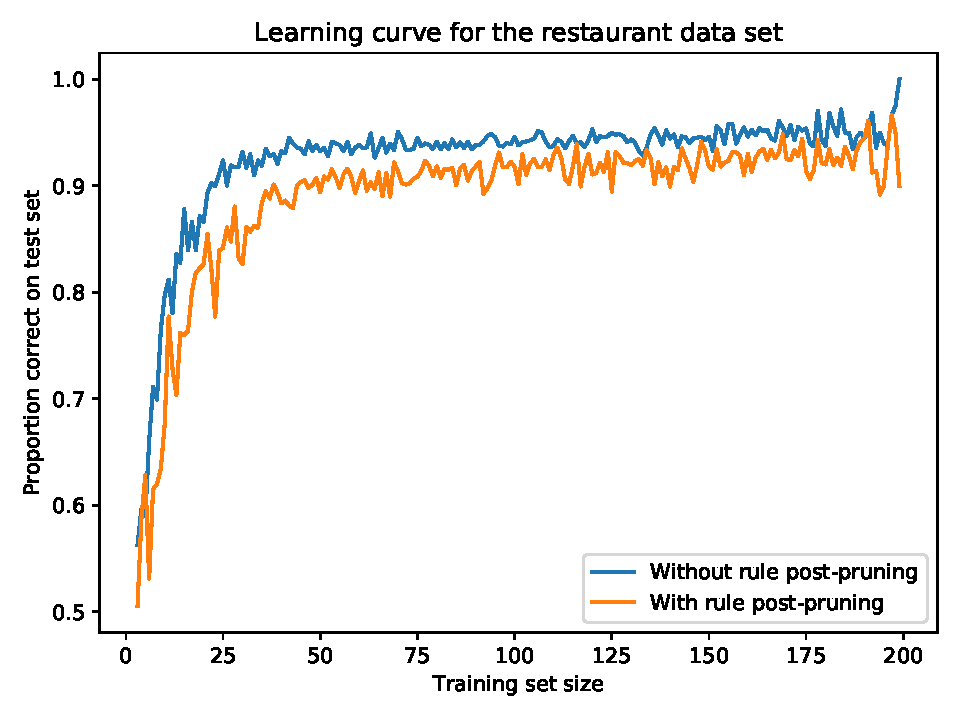
\includegraphics[width=\textwidth]{restaurant_4min.pdf}      
		\end{subfigure}    
		\hfill
		\begin{subfigure}{0.45\textwidth} 
			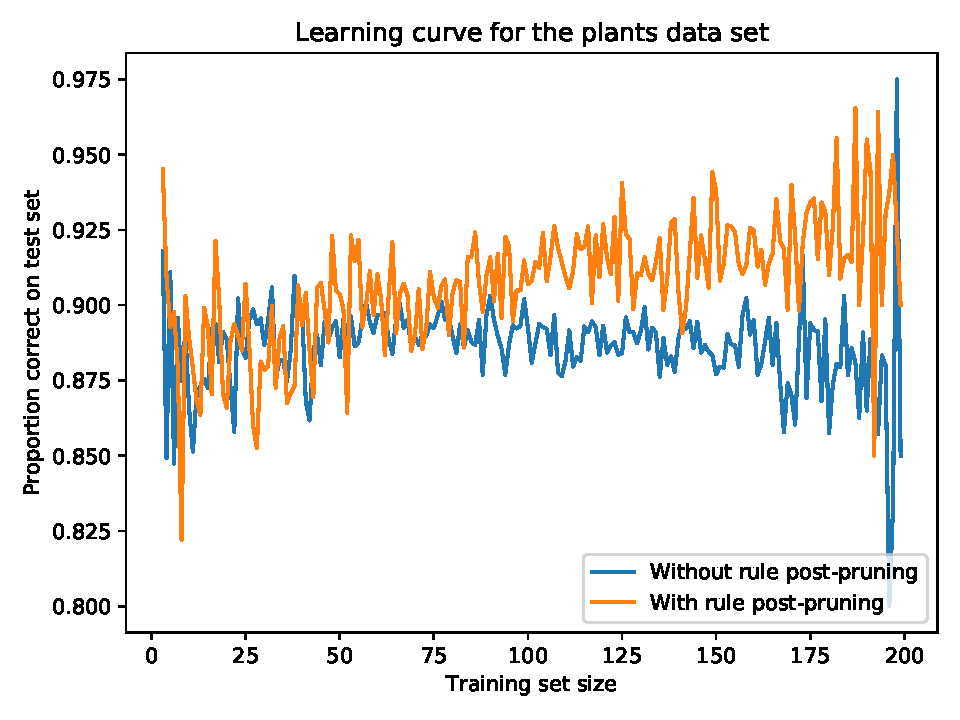
\includegraphics[width=\textwidth]{plants_5min.pdf}    
		\end{subfigure}    
	
		\begin{subfigure}{0.45\textwidth} 
			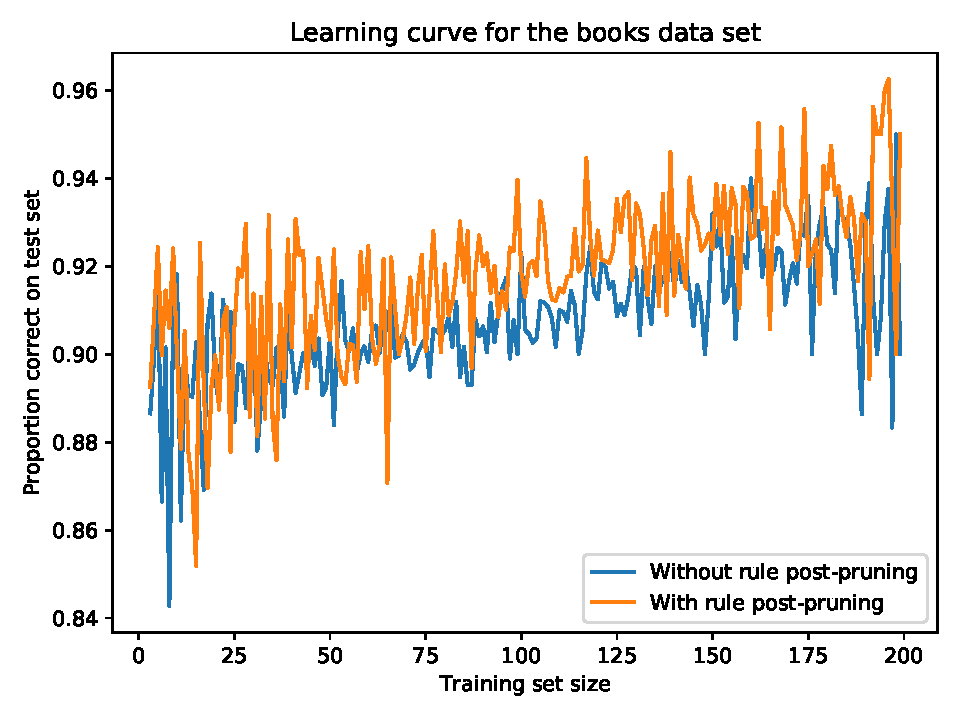
\includegraphics[width=\textwidth]{books_6min.pdf}       
		\end{subfigure}    
		\hfill
		\begin{subfigure}{0.45\textwidth} 
			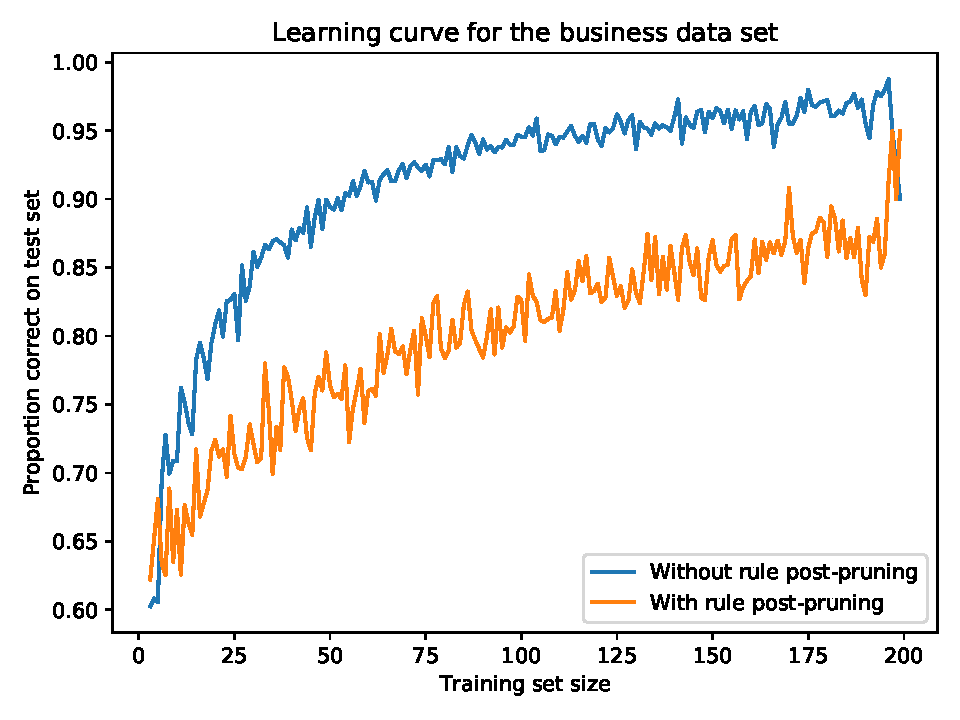
\includegraphics[width=\textwidth]{business_7min.pdf}       
		\end{subfigure}   
		\caption{Curve di apprendimento con 200 esempi estratti dai data set \restaurant{} (4 minuti), \plants{} (5 minuti), \books{} (6 minuti) e \business{} (7 minuti)}
		\label{fig:curva}
	\end{figure}
	
	\subsection{$K$-fold cross-validation} \label{sec:cross}
	Il file \texttt{cross\_validation\_test.py} calcola l'accuratezza dei due algoritmi di apprendimento rispetto al test set applicando una \emph{$k$-fold cross-validation}, con $k=10$: si eseguono 10 round di apprendimento, in ciascuno dei quali $1/10$ degli esempi è utilizzato come test set e il resto come training set, e si calcola la media dei 10 valori di accuratezza prodotti.
	
	Un esempio dei risultati ottenibili è mostrato in tabella \ref{tab:cross}.
	
	\begin{table}[t]
		\centering
		\begin{tabular}{|c|c|c|c|c|}
			\hline
			\multirow{2}{*}{Data Set} & \multicolumn{2}{|c|}{Accuratezza} & \multicolumn{2}{|c|}{Tempo (secondi)} \\
			\cline{2-5}
			& senza potatura & con potatura & senza potatura & con potatura \\
			\hline
			\restaurant & 0.997 & 0.961 & 0.104 & 7.767 \\
			\hline
			\plants & 0.934 & 0.945 & 0.396 & 446.565 ($\approx7\,$min) \\
			\hline
			\books & 0.941 & 0.942 & 0.337 & 841.848 ($\approx14\,$min) \\
			\hline
			\business & 0.999 & 0.974 & 0.158 & 52.778 \\
			\hline
		\end{tabular}
		\caption{Risultati di una 10-fold cross-validation su 1000 esempi di \restaurant, 2691 di \plants, 2687 di \books{} e 1257 di \business}
		\label{tab:cross}
	\end{table}
	
	\begin{thebibliography}{9}
		\bibitem{aima}
			Stuart Russel and Peter Norvig.
			\emph{Artificial Intelligence: A Modern Approach}.
			Third Edition.
			Pearson, 2010.
		\bibitem{mld}
		MLData repository. \textsc{url}: \url{http://mldata.org}
	
	\end{thebibliography}









































\end{document}